%%%%%%%%%%%%%%%%%%%%%%%%%%%%%%%%%%%%%%%%%
% Beamer Presentation
% LaTeX Template
% Version 1.0 (10/11/12)
%
% This template has been downloaded from:
% http://www.LaTeXTemplates.com
%
% License:
% CC BY-NC-SA 3.0 (http://creativecommons.org/licenses/by-nc-sa/3.0/)
%
%%%%%%%%%%%%%%%%%%%%%%%%%%%%%%%%%%%%%%%%%

%----------------------------------------------------------------------------------------
%	PACKAGES AND THEMES
%----------------------------------------------------------------------------------------

\documentclass{beamer}

\mode<presentation> {

% The Beamer class comes with a number of default slide themes
% which change the colors and layouts of slides. Below this is a list
% of all the themes, uncomment each in turn to see what they look like.

%\usetheme{default}
%\usetheme{AnnArbor}
%\usetheme{Antibes}
%\usetheme{Bergen}
%\usetheme{Berkeley}
%\usetheme{Berlin}
%\usetheme{Boadilla}
% \usetheme{CambridgeUS}
%\usetheme{Copenhagen}
%\usetheme{Darmstadt}
%\usetheme{Dresden}
%\usetheme{Frankfurt}
%\usetheme{Goettingen}
%\usetheme{Hannover}
%\usetheme{Ilmenau}
%\usetheme{JuanLesPins}
%\usetheme{Luebeck}
\usetheme{Madrid}
%\usetheme{Malmoe}
%\usetheme{Marburg}
%\usetheme{Montpellier}
% \usetheme{PaloAlto}
%\usetheme{Pittsburgh}
%\usetheme{Rochester}
%\usetheme{Singapore}
%\usetheme{Szeged}
%\usetheme{Warsaw}

% As well as themes, the Beamer class has a number of color themes
% for any slide theme. Uncomment each of these in turn to see how it
% changes the colors of your current slide theme.

%\usecolortheme{albatross}
%\usecolortheme{beaver}
%\usecolortheme{beetle}
%\usecolortheme{crane}
%\usecolortheme{dolphin}
%\usecolortheme{dove}
%\usecolortheme{fly}
%\usecolortheme{lily}
%\usecolortheme{orchid}
\usecolortheme{rose}
%\usecolortheme{seagull}
%\usecolortheme{seahorse}
%\usecolortheme{whale}
%\usecolortheme{wolverine}

%\setbeamertemplate{footline} % To remove the footer line in all slides uncomment this line
%\setbeamertemplate{footline}[page number] % To replace the footer line in all slides with a simple slide count uncomment this line

%\setbeamertemplate{navigation symbols}{} % To remove the navigation symbols from the bottom of all slides uncomment this line
}

\usepackage{graphicx} % Allows including images
\graphicspath{{./fig/}}
\DeclareGraphicsExtensions{.pdf,.jpeg,.png}
\usepackage{booktabs} % Allows the use of \toprule, \midrule and \bottomrule in tables
\usepackage[numberedbib]{apacite}
\usepackage{ amssymb }

%----------------------------------------------------------------------------------------
%	TITLE PAGE
%----------------------------------------------------------------------------------------

\title[ContCtrl with deepRL (Lilicrap, 2016)] {
    Continuous control with deep reinforcement learning
    \vspace{5mm}
    (DeepRL Reading, RDL, UQ)
}

\author{Vektor Dewanto} % Your name
\institute[RDL, UQ] % Your institution as it will appear on the bottom of every slide, may be shorthand to save space
{
% Affiliation: RDL, UQ\\ % Your institution for the title page
\medskip
\textit{vektor.dewanto@gmail.com } % Your email address
}
\date{\today} % Date, can be changed to a custom date

\begin{document}

\begin{frame}
\titlepage % Print the title page as the first slide
\end{frame}

\begin{frame}
\frametitle{Outline} % Table of contents slide, comment this block out to remove it
\tableofcontents % Throughout your presentation, if you choose to use \section{} and \subsection{} commands, these will automatically be printed on this slide as an overview of your presentation
\end{frame}

%----------------------------------------------------------------------------------------
%	PRESENTATION SLIDES
%----------------------------------------------------------------------------------------
%%%%%%%%%%%%%%%%%%%%%%%%%%%%%%%%%%%%%%%%%%%%%%%%%%%%%%%%%%%%%%%%%%%%%%%%%%%%%%%
\section{Introduction}
\frame{\tableofcontents[currentsection, hideothersubsections]}

\begin{frame}
\frametitle{Introduction}

\begin{figure}
    \centering
    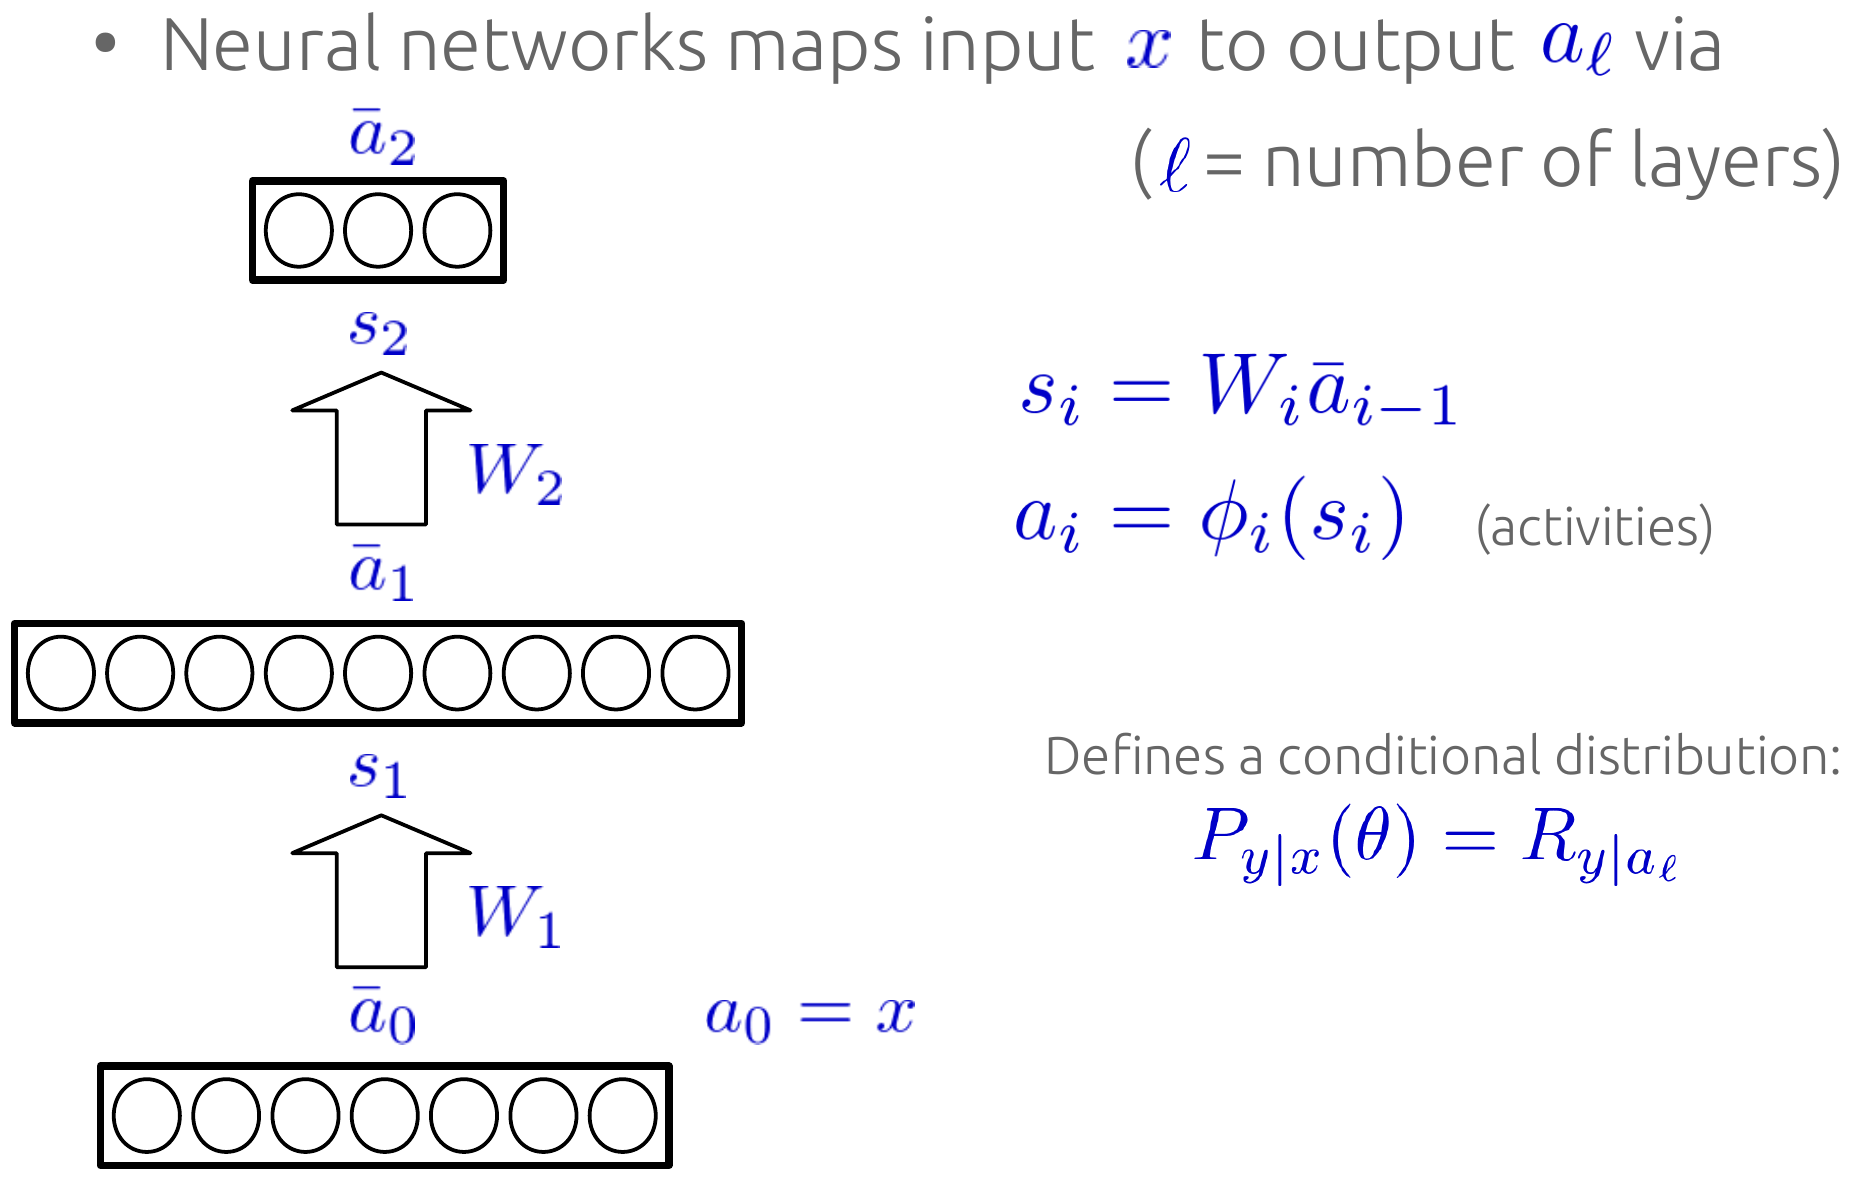
\includegraphics[scale=0.2]{net}
\end{figure}

\begin{itemize}
    \item $\bar{a}_i$ is $a_i$ appended by a homogeneous coordinate with value 1, ie
            to capture bias parameters explicitly
\end{itemize}
\end{frame}

\begin{frame}
\frametitle{Introduction}

\begin{figure}
    \centering
    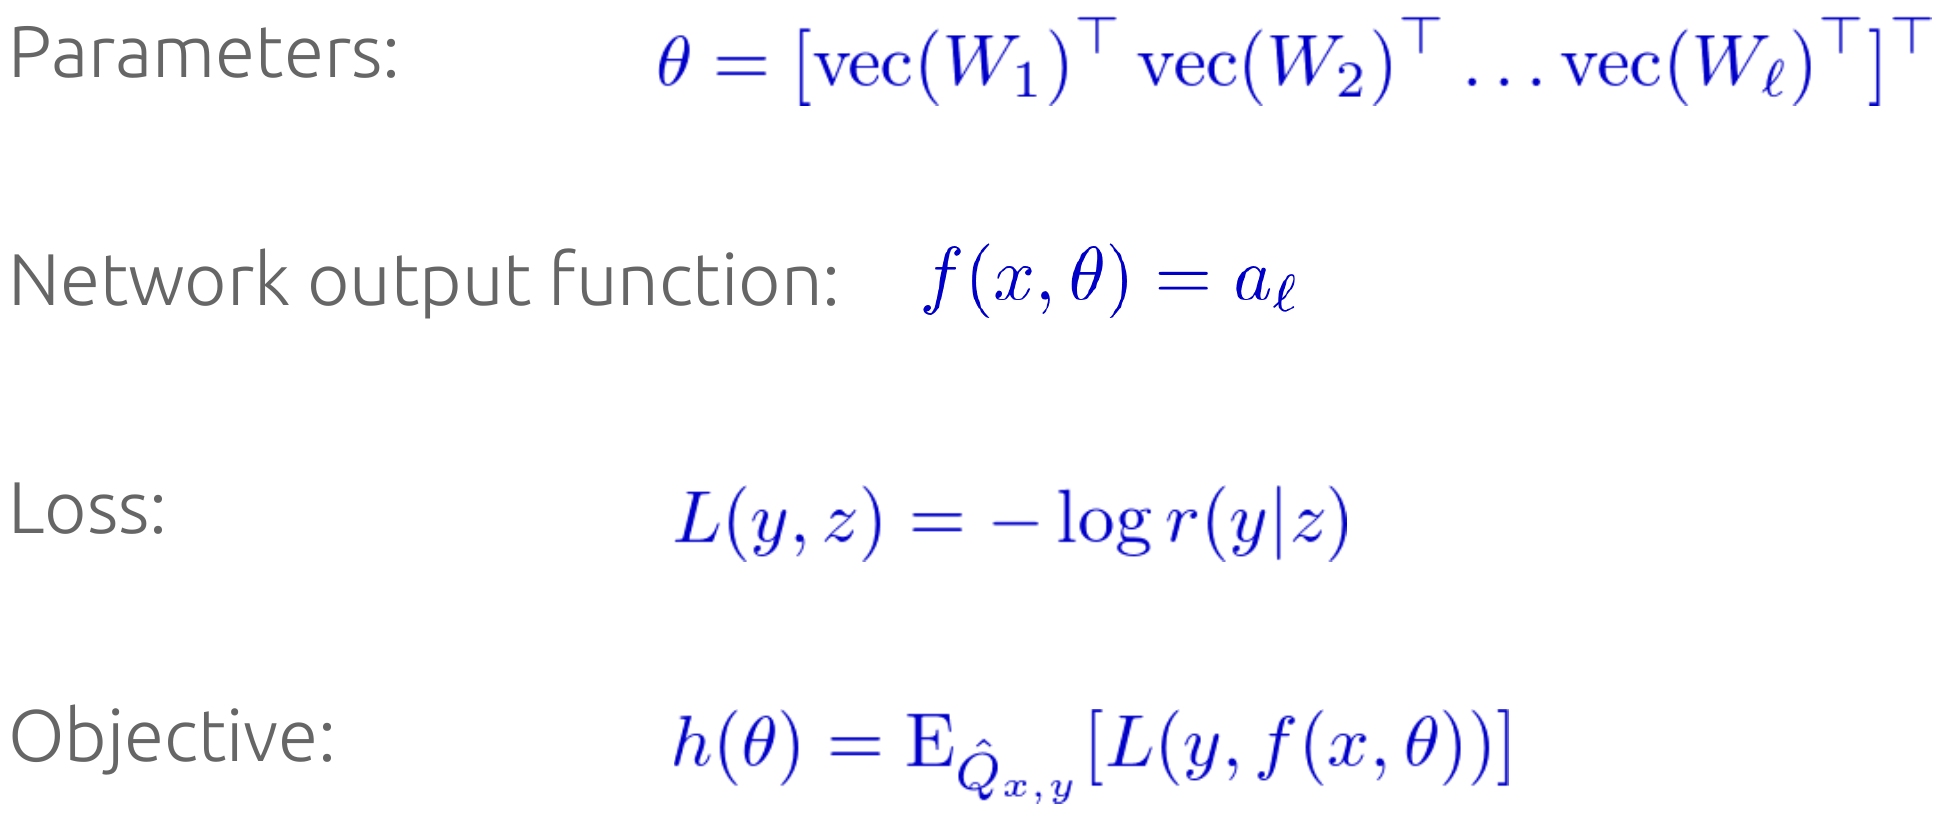
\includegraphics[scale=0.2]{net_param}
\end{figure}

\begin{itemize}
    \item $vec$ vectorizes matrices by stacking their columns together
    \item $\hat{Q}_{x, y}$ is a training distribution
    \item $p(y|x, \theta) = r(y|f(x, \theta))$ is the density function of $P_{y|x}(\theta) = R_{y|f(x,\theta)}$
    \item minimizing $h(\theta)$ can be seen as maximum likelihood learning of~$P_{y|x}(\theta)$.
\end{itemize}

\end{frame}

\begin{frame}
\frametitle{Introduction}
Newton-type update: $\theta_{k+1} = \theta_k - \alpha_k (\nabla^2 h)^{-1} \nabla h$
% \begin{itemize}
%     \item Newton-type update: $\theta_{t+1} = \theta_t - \alpha (\nabla^2 h)^{-1} \nabla h$
% \end{itemize}
\begin{figure}
    \raggedright
    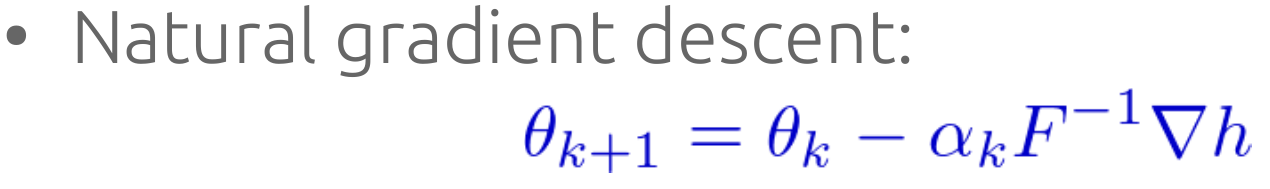
\includegraphics[scale=0.25]{natgrad}
\end{figure}

\begin{figure}
    \raggedright
    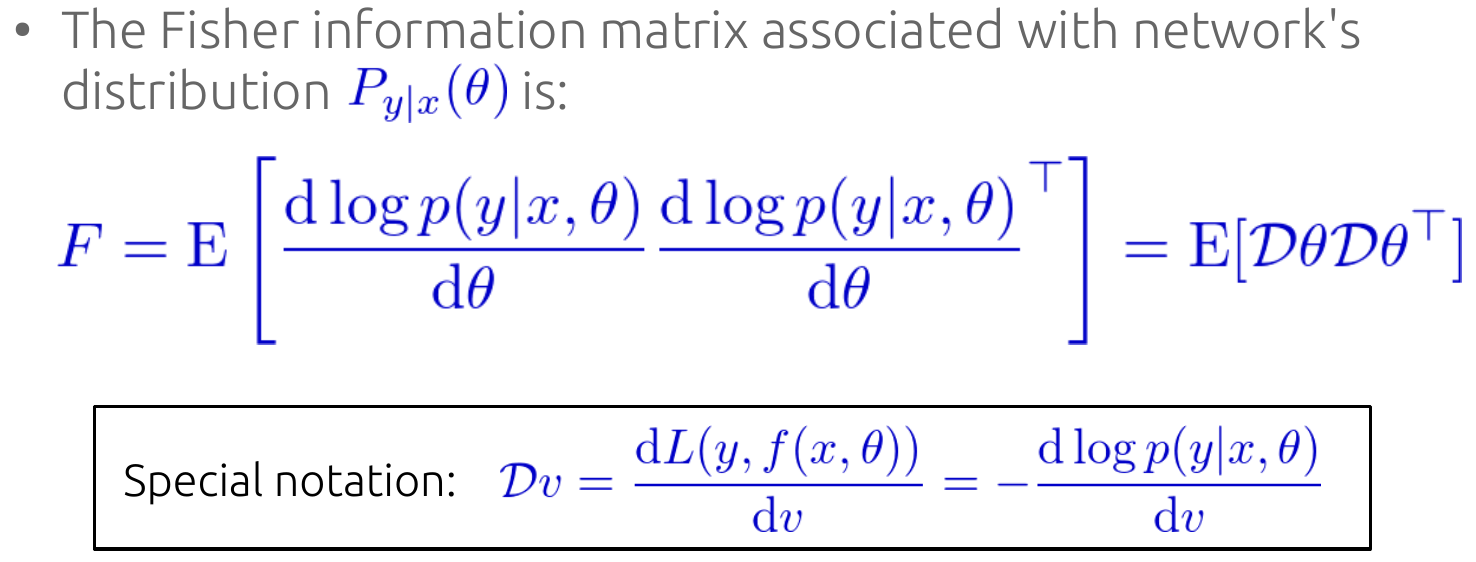
\includegraphics[scale=0.25]{fisher}
\end{figure}

\end{frame}

\section{Background}
\frame{\tableofcontents[currentsection, hideothersubsections]}

\begin{frame}
\frametitle{Background: MDP}
\textbf{The environment}, $E$: \\
a Markov decision process with a state space $S$, action space $A = \mathbb{R}^N$,
an initial state distribution $p(s_1)$, transition dynamics $p(s_{t+1}|s_t, a_t)$, and
reward function $r(s_t, a_t)$.
\vspace{2.5mm}

\textbf{At each discrete timestep} $t$, \\
the agent receives an observation $x_t = s_t$ (fully observable),
takes an action $a_t$ and receives a scalar reward $r_t$.
\vspace{2.5mm}

\textbf{The return from a state}: \\
$R_t= \sum_{i=t}^T  \gamma^{(i-t)} r(s_i, a_i)$ with a discounting factor $\gamma \in [0, 1]$.
\vspace{2.5mm}

\textbf{Goal}: \\
to learn a policy, $\pi: S \mapsto P(A)$, which
maximizes $J = \mathbb{E}_{r_i,s_i \sim E,a_i \sim \pi} [R_1]$.
\vspace{2.5mm}

\textbf{Action-value function}:\\
$Q^{\pi}(s_t,a_t) = \mathbb{E}_{r_{i \ge t},s_{i>t} \sim E,a_{i>t} \sim \pi} [R_t|s_t,a_t]$.
\end{frame}

\begin{frame}
\frametitle{Background: MDP with deterministic policy}
Bellman equation (the recursive relationship):
\begin{equation}
Q^{\pi} (s_t,a_t) = \mathbb{E}_{r_{t},s_{t+1} \sim E} \Big[ r(s_t,a_t) + \gamma \mathbb{E}_{a_{t+1} \sim \pi} [Q^{\pi}(s_{t+1},a_{t+1})] \Big]
\end{equation}

If the target policy is deterministic, $\mu: S \mapsto A$, then:
\begin{equation}
Q^{\mu} (s_t,a_t) = \mathbb{E}_{r_{t},s_{t+1} \sim E} \Big[ r(s_t,a_t) + \gamma Q^{\mu}(s_{t+1},\mu(s_{t+1})) \Big]
\end{equation}

Thus:
\begin{itemize}
\item the expectation depends only on the environment $E$,
\item possible to learn $Q^{\mu}$ off-policy, using transitions which
are generated from a different stochastic behavior policy $\beta$.
\end{itemize}
\end{frame}

\begin{frame}
\frametitle{Background: Fn approximator}
Consider fn approximators parameterized by $\theta^Q$, \\
which we optimize by minimizing the loss:
\begin{equation} \label{equ:qloss}
L(\theta^Q) =\mathbb{E}_{s_t \sim \rho^{\beta}, a \sim \beta, r_t \sim E} \Big[ \Big( Q (s_t,a_t|\theta^Q) - y_t \Big)^2 \Big]
\end{equation}
where:\\
$y_t = r(s_t,a_t) + \gamma Q(s_{t+1},\mu(s_{t+1}) | \theta^Q)$, and \\
$\rho^{\beta}$: the discounted state visitation distribution for a policy $\beta$.
\vspace{5mm}

Typically, ignore the fact that $y_t$ is also dependent on $\theta^Q$.\\
\end{frame}

\begin{frame}
\frametitle{Background: Actor-critic approach}
\begin{figure}
    \centering
    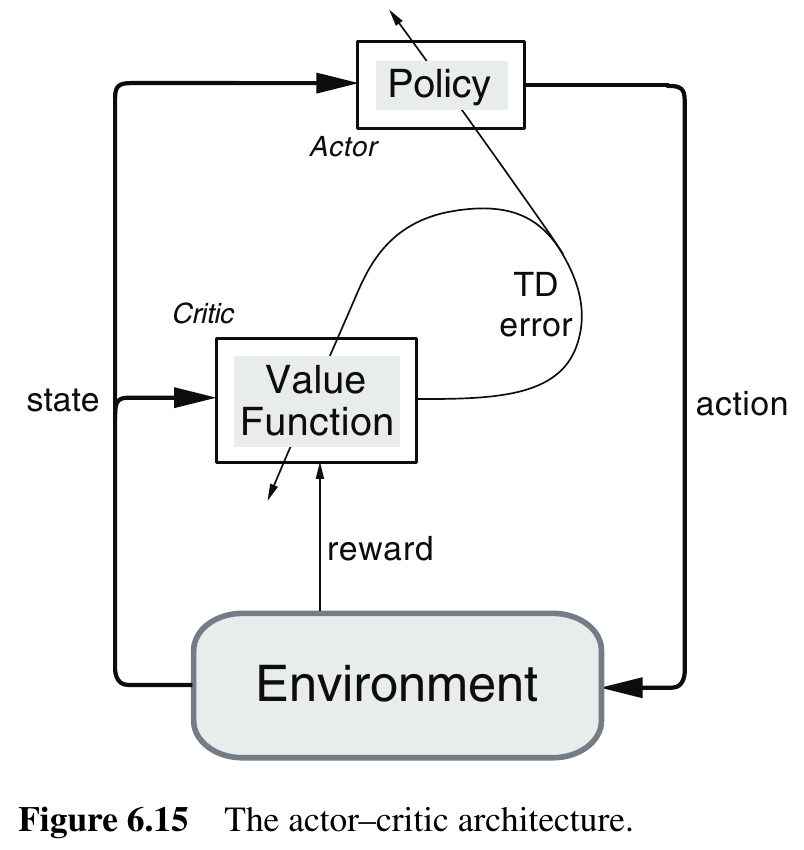
\includegraphics[scale=0.35]{actorcritic_arch}
\end{figure}
\end{frame}

% \begin{frame}
% \frametitle{Background: Actor-critic \cite{Sutton1998}}
% The Actor-Critic Algorithm is essentially a hybrid method to combine the policy gradient method and the value function method together.
% The policy function is known as the actor, while the value function is referred to as the critic.
% Essentially, the actor produces the action aa given the current state of the environment ss, while the critic produces a signal to criticizes the actions made by the actor.
% \end{frame}

% deep Q-network:
% \begin{itemize}
%   \item innovation:
%   \begin{itemize}
%     \item the network is trained off-policy with samples from a replay buffer to minimize correlations between samples;
%     the use of a replay buffer
%     \item the network is trained with a target Q network to give consistent targets during temporal difference backups.
%     a separate target network for calculating $y_t$
%   \end{itemize}
%   \item able to:
%   \begin{itemize}
%     \item solves problems with high-dimensional observation spaces,
%     \item can only handle discrete and low-dimensional action spaces.
%   \end{itemize}
% \end{itemize}

\section{Methods}
\frame{\tableofcontents[currentsection, hideothersubsections]}

\begin{frame}
\frametitle{Methods: Deep DPG}
\begin{figure}
    \centering
    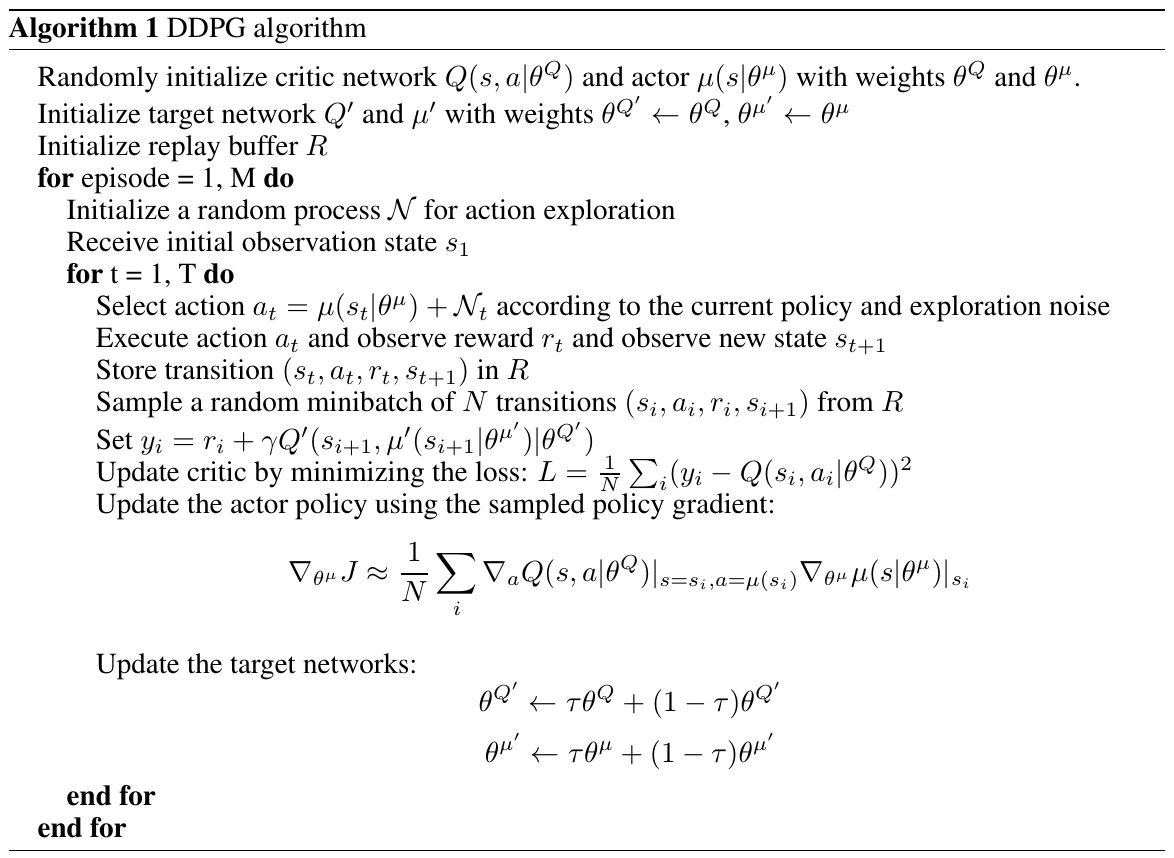
\includegraphics[scale=0.25]{ddpg_algo}
\end{figure}

{\footnotesize
Deep DPG (=DPG+DQN) components:
\begin{itemize}
  \item Deterministic Policy-Gradient (DPG) \cite{Silver2014}
  \item Deep Q-Network (DQN= QLearning + deepLearning) {\scriptsize\cite{Mnih2013}}
  \item Actor-Critic Methods \cite{Sutton1998}
\end{itemize}
}
\end{frame}

\begin{frame}
\frametitle{Methods: DPG \cite{Silver2014}}

DPG: Deterministic Policy Gradient, an actor-critic approach:
\begin{itemize}
  \item actor: $\mu (s|\theta^{\mu})$,
  specifies the current policy by deterministically mapping states to a specific action
  \item critic: $Q(s, a)$,
  learned using the Bellman equation as in Q-learning.
\end{itemize}
\vspace{3mm}

Update $\theta^{\mu}$ by applying the chain rule to the expected return from
the start distribution, $J$, with respect to the actor parameters, $\theta^{\mu}$:
\begin{equation} \label{equ:policy_grad}
\begin{split}
\nabla_{\theta^{\mu}} J &  \approx \mathbb{E}_{s_t \sim \rho^{\beta}} \Big[ \nabla_{\theta^{\mu}} Q(s,a|\theta^Q) |_{s = s_t, a = \mu(s_t|\theta^{\mu})} \Big] \\
  & = \mathbb{E}_{s_t \sim \rho^{\beta}} \Big[ \nabla_{\theta^{\mu}} Q(s,a|\theta^Q) |_{s = s_t, a = \mu(s_t)} \nabla_{\theta^{\mu}} \mu(s|\theta^{\mu})|_{s = s_t} \Big]
\end{split}
\end{equation}

Equ.~\ref{equ:policy_grad} is the policy gradient (the gradient of the policy's performance),
in practice the discount in $\rho^{\beta}$ is ignored.
\end{frame}

\begin{frame}
\frametitle{Methods: Replay-buffer, as in DQN~\cite{Mnih2013}}
Why:
\begin{itemize}
\item NeuralNets assume iid samples;\\
the samples from exploring sequentially in an environment are \textbf{not} iid
\item to make efficient use of hardware optimizations:\\
to learn in minibatches rather than (fully) online
\end{itemize}
\vspace{5mm}

How:
\begin{itemize}
  \item replay buffer, $R$, contains $(s_t, a_t, r_t, s_{t+1})$ sampled from $E$ using an exploration policy
  \item At each timestep the actor and critic are updated by sampling a minibatch uniformly from the buffer
% Because DDPG is an off-policy algorithm, the replay buffer can be large, allowing the algorithm to benefit from learning across a set of uncorrelated transitions.
\end{itemize}

\end{frame}

\begin{frame}
\frametitle{Methods: Fix target network, {\footnotesize as in DQN~\cite{Mnih2013}}}
Why:
\begin{itemize}
\item Q-learning (eq.\ref{equ:qloss}) with NeuralNets is unstable, \\
since the network $Q(s, a|\theta^Q)$ being updated is also used in
calculating the target value, $y$
\end{itemize}
\vspace{5mm}

How:
\begin{itemize}
\item {\footnotesize create a copy of the actor and critic networks, i.e.}
  $Q'(s, a|\theta^{Q'})$ and $\mu'(s|\theta^{\mu'})$
\item use $Q'(s, a|\theta^{Q'})$ and $\mu'(s|\theta^{\mu'})$ for calculating the target values
\item target networks update: \\
    $\theta' \leftarrow \tau \theta + (1 - \tau) \theta'$ with $\tau \ll 1$\\
    (warn: may slow learning, since the target network delays the propagation of value estimations, but
    in practice, this was greatly outweighed by the stability of learning)
\end{itemize}

\end{frame}


\begin{frame}
\frametitle{Methods: Feature scaling: batch normalization}
Why:
\begin{itemize}
\item different components of the observation may have different physical units (for example, positions versus velocities)
\item their ranges may vary across environments
% \item make it difficult
%   a) for the network to learn effectively
%   b) to find hyper-parameters which generalise across environments with different scales of state values.
% \item to minimize covariance shift during training, by ensuring that each layer receives whitened input
\end{itemize}
\vspace{5mm}

How:
\begin{itemize}
\item normalizes each dimension across the samples in a minibatch to have unit mean and variance.
\item maintains a running average of the mean and variance to use for normalization during testing
(during xploration or evaluation)
\end{itemize}

\end{frame}

\begin{frame}
\frametitle{Methods: Exploration}
Why:\\
Exploration-exploitation dillema
\vspace{5mm}

How:\\
\begin{itemize}
\item Construct an exploration policy $\mu^{xplor}$ by adding noise sampled from
a noise process $\mathcal{N}$ to our actor policy:
$\mu^{xplor} = \mu(s_t | \theta^{\mu}_t) + \mathcal{N}$.\\
\item Here, $\mathcal{N}$ is from Ornstein-Uhlenbeck process,\\
to generate temporally correlated exploration for exploration efficiency in physical control problems with inertia.
\end{itemize}
\end{frame}

\begin{frame}
\frametitle{Methods: Deep DPG Algo}
\begin{figure}
    \centering
    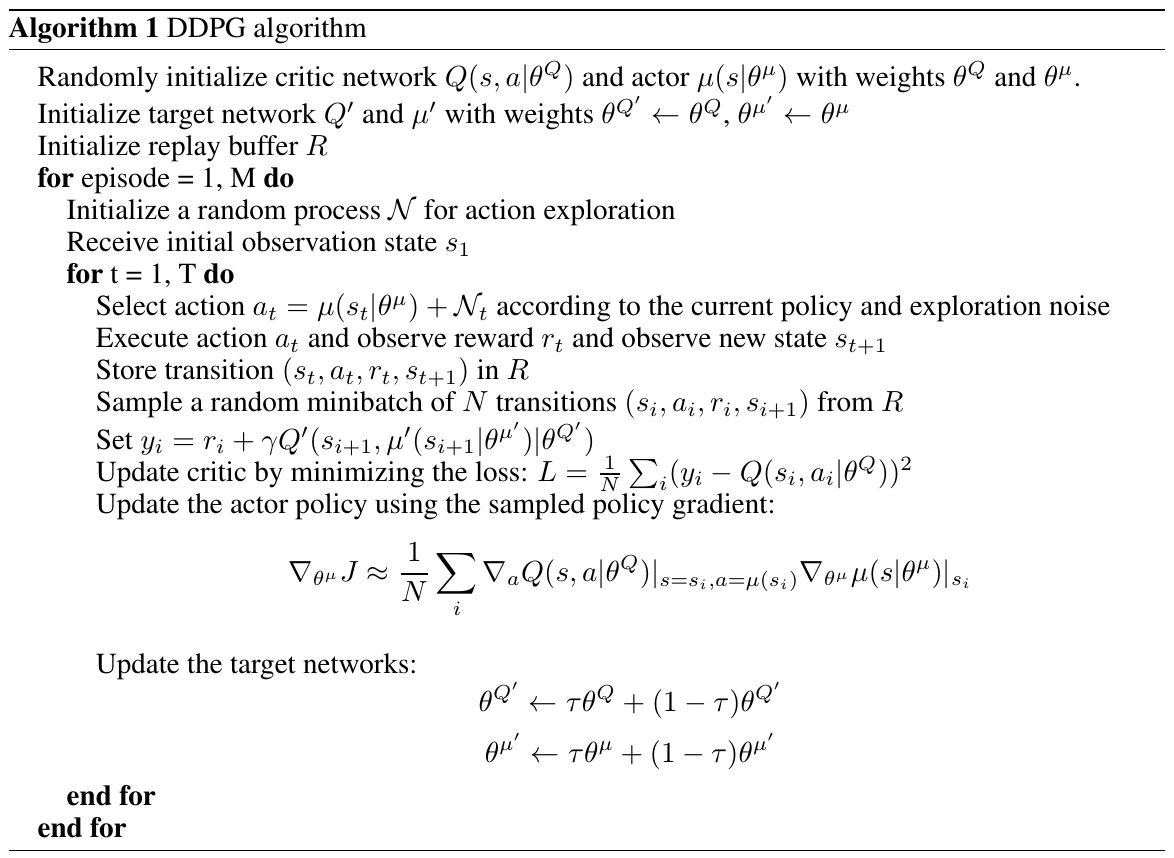
\includegraphics[scale=0.35]{ddpg_algo}
\end{figure}
\end{frame}

\section{Setup}
\frame{\tableofcontents[currentsection, hideothersubsections]}

\begin{frame}
\frametitle{Experiment Setup: Tasks}

\begin{figure}
    \centering
    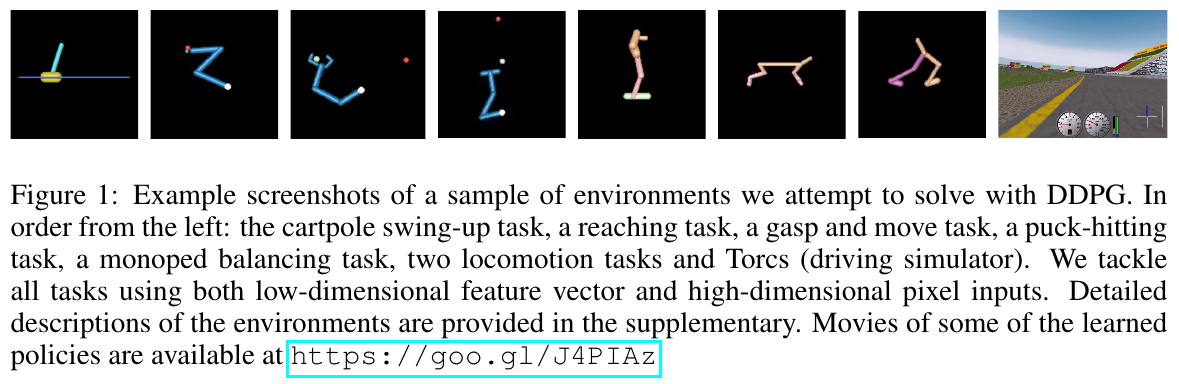
\includegraphics[scale=0.3]{fig_1}
\end{figure}

\begin{itemize}
  \item 20 simulated physics task, including:
  \begin{itemize}
    \item gripperRandom:
    Agent must use an arm with gripper appendage to grasp an object and manuver the object, which
    are initialized in random locations
    % \item reacher3daRandomTarget:
    % Agent is required to move a 7-DOF human-like arm from random starting locations to random target positions.
    \item reacherObstacle:
    Agent is required to move a 5-DOF arm around an obstacle to a randomized target position.
  \end{itemize}
  \item features, both:
    \begin{itemize}
    \item a low-dimensional state description (such as joint angles and positions)
    \item high-dimensional renderings of the environment
  \end{itemize}
\end{itemize}

\end{frame}

\begin{frame}
\frametitle{Experiment Setup: Tasks}

\begin{figure}
    \centering
    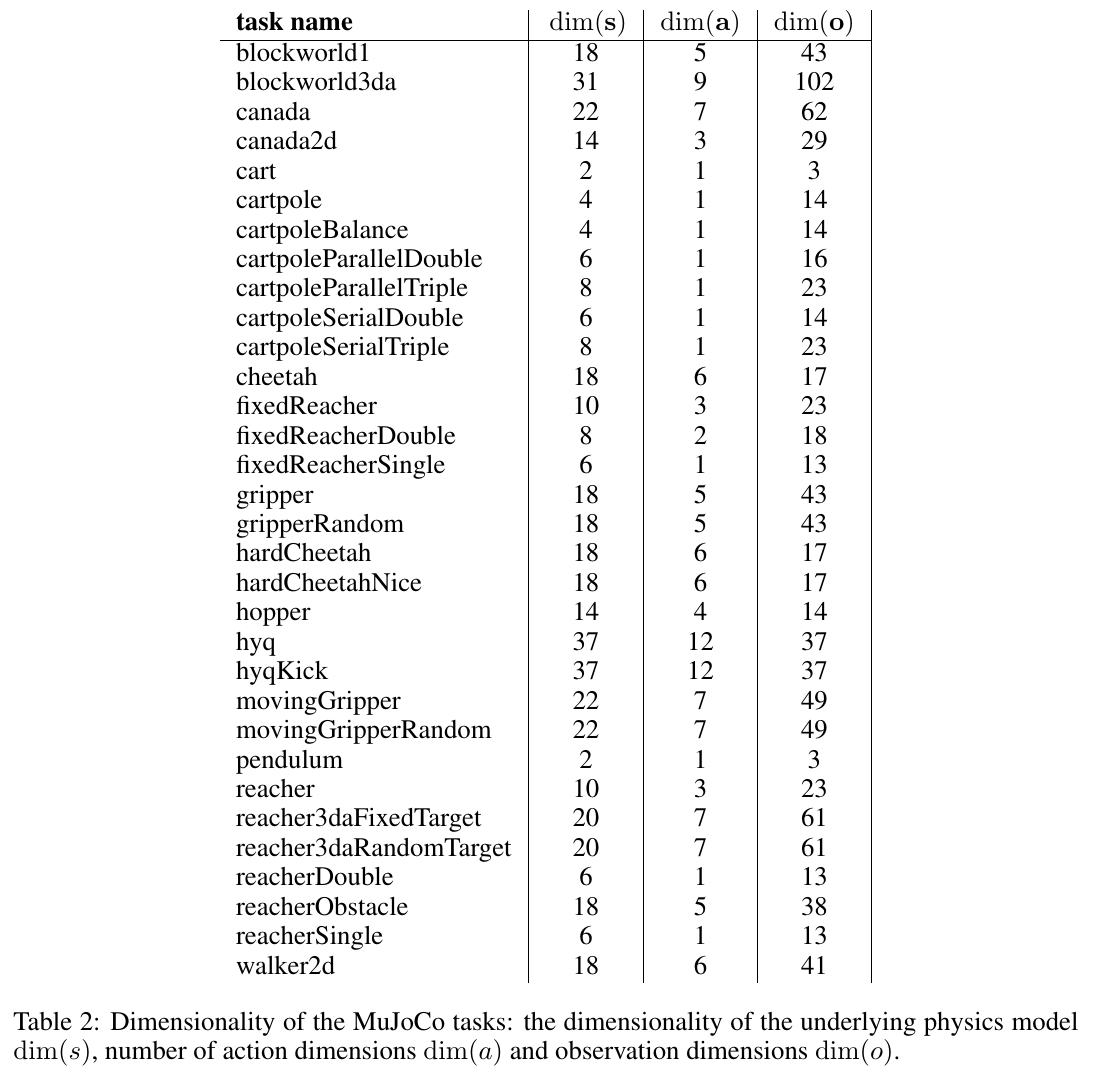
\includegraphics[scale=0.25]{task_dim}
\end{figure}

\end{frame}


\begin{frame}
\frametitle{Experiment Setup: Baseline, Assumptions}

Assumption:
\begin{itemize}
  \item env is MDP, the environment is fully-observed
\end{itemize}

Baseline:
\begin{itemize}
  \item 2 types:
  \begin{itemize}
    \item \textbf{naive policy:} the mean return from a naive policy which samples actions from
    a uniform distribution over the valid action space;
    \item \textbf{iLQG~\cite{Todorov2005}}: a planning based solver with full access to
    the underlying physical model and its derivatives.
  \end{itemize}
  \item normalize baseline scores so that
    \begin{itemize}
    \item \textbf{naive policy}: has a mean score of 0
    \item \textbf{iLQG}: has a mean score of 1
  \end{itemize}
\end{itemize}

\end{frame}


\section{Results}
\frame{\tableofcontents[currentsection, hideothersubsections]}

\begin{frame}
\frametitle{Results: Performance, 5 runs, score: naive= 0, iLQG= 1}
\begin{figure}
    \centering
    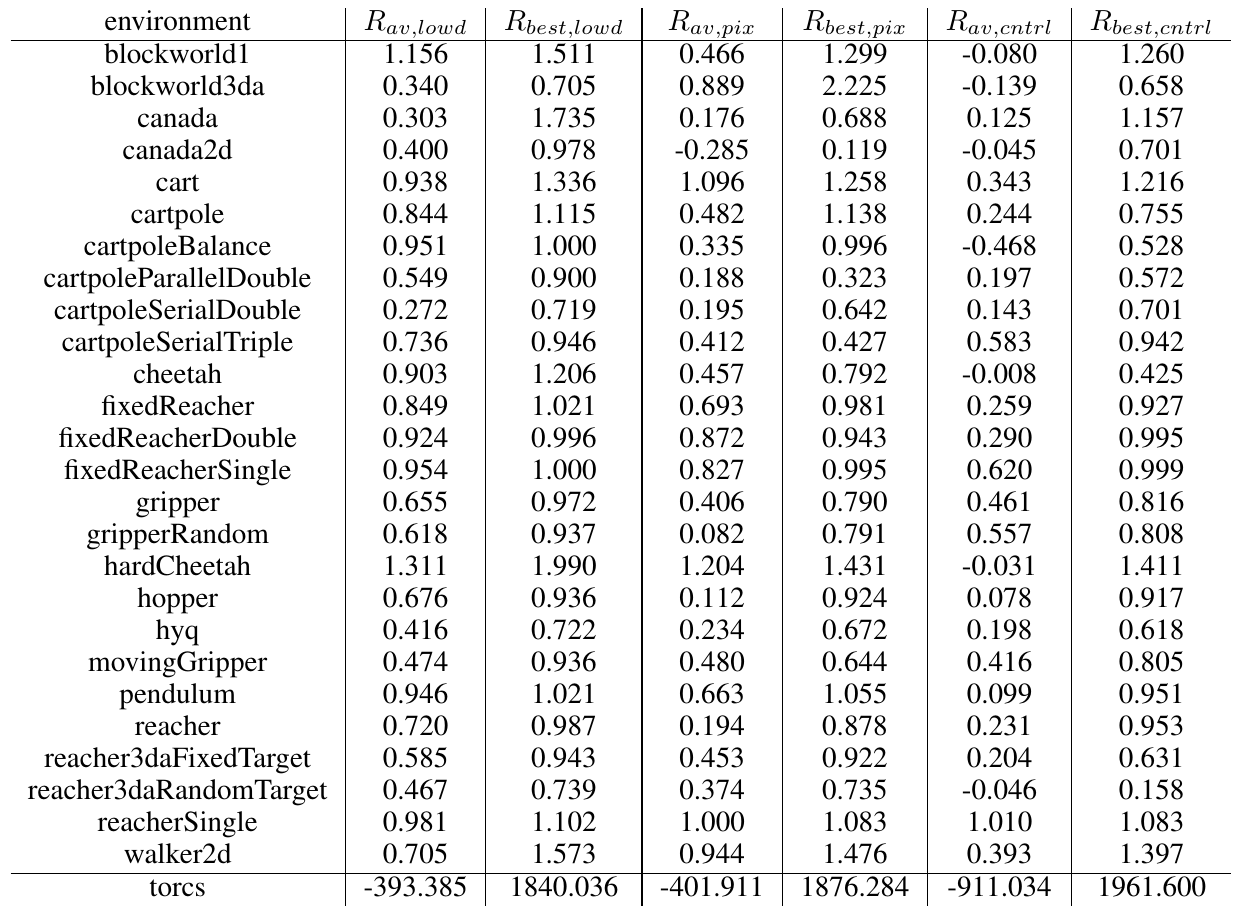
\includegraphics[scale=0.3]{perf_table}
\end{figure}
\end{frame}

\begin{frame}
\frametitle{Results: Estimated Q values}
% \begin{figure}
%     \centering
%     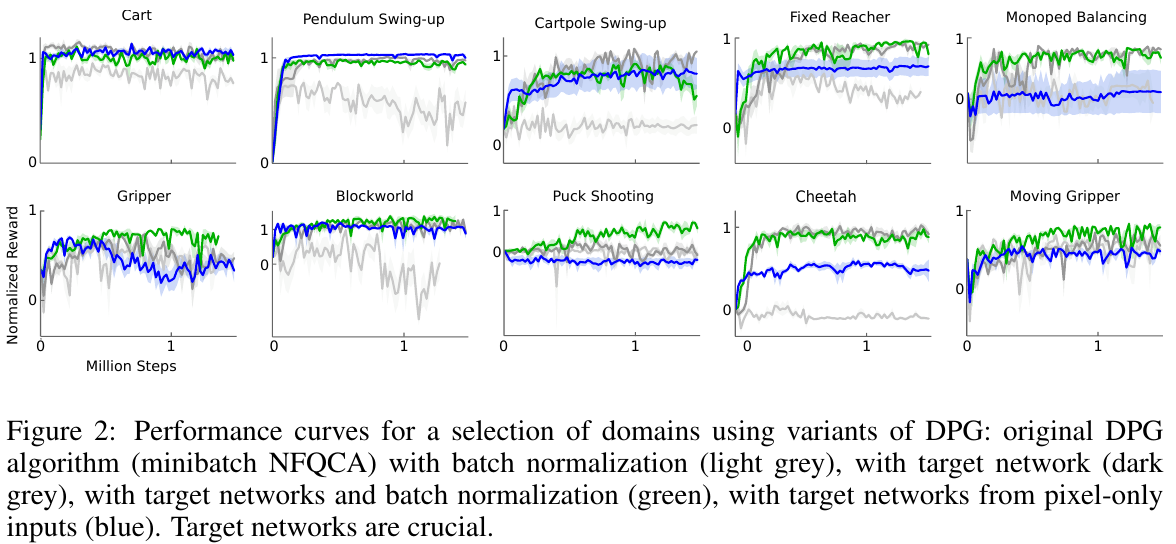
\includegraphics[scale=0.3]{fig_2}
% \end{figure}

\begin{figure}
    \centering
    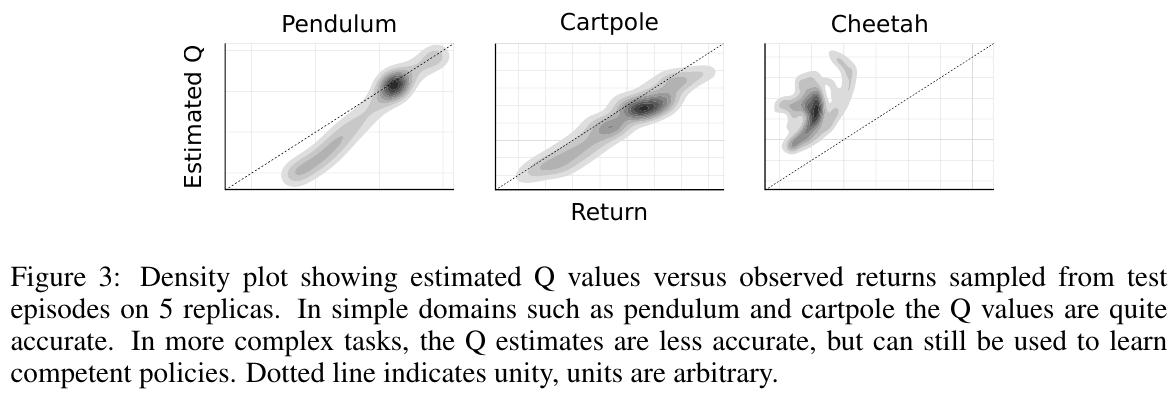
\includegraphics[scale=0.35]{fig_3}
\end{figure}

\end{frame}

\begin{frame}
\frametitle{Results: In words...}

\begin{itemize}
  \item able to find policies whose performance is \textbf{competitive} \\
  with those found by a planning algorithm with full access to the dynamics of the domain and its derivatives.
  \item for many of the tasks the algorithm, can learn policies end-to-end: directly from raw pixel inputs.
  \item in some simpler tasks, learning policies from pixels is just as fast as learning using the low-dimensional state descriptor.\\
  (may also be that the convolutional layers provide an easily separable representation of state space,
  which is straightforward for the higher layers to learn on quickly)
\end{itemize}

See: supplemental video!
\end{frame}

\section{Conclusions}
\frame{\tableofcontents[currentsection, hideothersubsections]}

\begin{frame}
\frametitle{Conclusions}
?
\end{frame}

\begin{frame}
\Huge{\centerline{Discussion time and thank you.}}
\end{frame}
% \section{My Current Work}
\frame{\tableofcontents[currentsection, hideothersubsections]}

\begin{frame}
\frametitle{My current work: Interest}

\begin{figure}
    \centering
    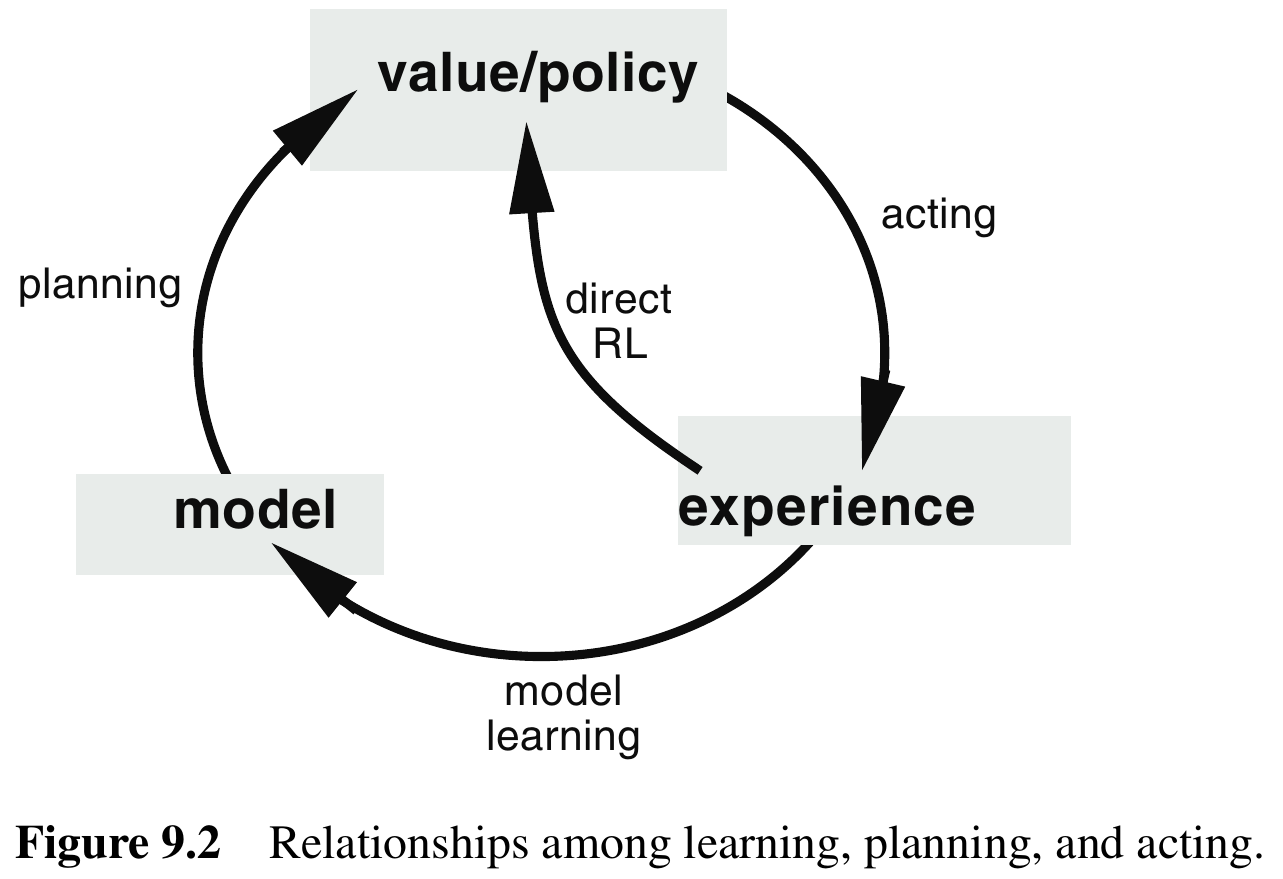
\includegraphics[scale=0.20]{learningplanning_arch}
\end{figure}

Interests, lack of ideas still :(
\begin{itemize}
  \item interaction of model-based and model-free RL, continuous control,
  deeply bayesian RL for POMDPs,
  \item physics-intensive tasks with real robots
\end{itemize}
\end{frame}

\begin{frame}
\frametitle{My current work: On going}
\begin{itemize}
  \item playing around with sim timestep, case: grasping
  \item movodemo, case: pickandplace
\end{itemize}
\vspace{5mm}

Enjoy: some videos!
\end{frame}

% \begin{frame}
% \frametitle{Interests: more detail}
% Nuts and Bolts Task:
% Assumed that the robot has already been trained to recognize, want, grasp, and eat cookies.
% The cookies in this task are within cages, and the cage covers are locked with nuts and bolts.
% The robot must learn to use a wrench and his fingers to remove the cover and get the cookie.
% \end{frame}

% Practical :
% \begin{itemize}
%   \item grasping, using tools,
%   e.g.  Nuts and Bolts Task:
%   \item navigation among movable obstacles
%   (motion planning with minimal collisions)
%   \item (physics) games, e.g
%   car racing, block stacking (simplified Tummple, Jenga)
% \end{itemize}

\begin{frame} [allowframebreaks]
\frametitle{References}
{\tiny
\bibliographystyle{apacite}
\bibliography{ref}
}
\end{frame}

\begin{frame}
\Huge{\centerline{Discussion time and thank you.}}
\end{frame}

%%%%%%%%%%%%%%%%%%%%%%%%%%%%%%%%%%%%%%%%%%%%%%%%%%%%%%%%%%%%%%%%%%%%%%%%%%%%%%%

\end{document}
